\documentclass{article}

% Language setting
\usepackage[spanish]{babel}

% Set page size and margins
\usepackage[letterpaper,top=2cm,bottom=2cm,left=3cm,right=3cm,marginparwidth=1.75cm]{geometry}

% Useful packages
\usepackage{amsmath}
\usepackage{graphicx}
\usepackage{pgfplots}
\pgfplotsset{compat=1.17}
\usepgfplotslibrary{fillbetween}
\usepackage[colorlinks=true, allcolors=customcolor]{hyperref}
\usepackage{fourier}
\usepackage{parskip}
\usepackage{comment}
\usepackage{listings}
\usepackage{float}
\usepackage{subcaption}
\usepackage{multicol}
\usepackage{makeidx}
\usepackage{booktabs}

\makeindex

\setlength{\textfloatsep}{10pt} % Ajusta el espacio entre texto y figuras flotantes
\definecolor{customcolor}{RGB}{69, 97, 140}
\definecolor{color1}{RGB}{3,103,166}
\definecolor{color2}{RGB}{79,115,2} 
\definecolor{color3}{RGB}{242,183,5} 
\definecolor{color4}{RGB}{166,41,13} 
\definecolor{color5}{RGB}{242,116,5} 


\title{Simulación de Objetos Deformables \\ \large{Práctica 4 - Curso 2023-24}}
\author{Miguel Cuevas Escrig \and Carlos Izquierdo Gil}
\date{\today}

\begin{document}
\maketitle
\tableofcontents
\section{Introducción}

El objetivo de esta práctica es la simulación de objetos deformables en un entorno físico. Se implementan dos modelos diferentes: un sistema dinámico y unsistema cinematico. El primero se basa en mallas deformables utilizando muelles y el segundo en movimientos de vértices en base a funciones de onda.


\section{Implementación}

\subsection{Malla deformable por muelles}\label{sec:malla-muelle}

Para consegír que la malla se deforme, se genera una estructura de partículas que se conectan entre sí mediante muelles en diferentes configuraciones. La fuerza elastica que se aplica a cada partícula es la suma de las fuerzas de los muelles que la conectan con otras partículas. Tambien se aplica una fuerza de amortiguamiento lineal para simular fricción.

La malla se construye a partir de una posición inicial, de su orientación en el espacio, de la cantidad de partículas en cada eje de esta y de la separación entre ellas.
\begin{lstlisting}[language=Java, frame=single]
    for (int j = 0; j < _numNodesV; j++)
    {
       for (int i = 0; i < _numNodesH; i++)
       {
          PVector pos = new PVector(
            initPos.x + i*_sepH * dir.x, 
            initPos.y + j * _sepV * dir.y, 
            initPos.z + j *_sepH* dir.z);

          PVector vel = new PVector(0, 0, 0);

          _nodes[i][j] = new Particle(pos,vel,M,false, false);
       }
    }
    
\end{lstlisting}

Una vez creada la estructura, se procede a instanciar los muelles segun la configuración deseada.

\begin{lstlisting}[language=Java, frame=single]
    switch (_springLayout) {
         case STRUCTURAL:
          addStructuralSprings();
          break;
         case SHEAR:
            addShearSprings();
            break;
         case BEND:
            addBendSprings();
            break;
         case STRUCTURAL_AND_SHEAR:
            addStructuralSprings();
            addShearSprings();
            break;
         case STRUCTURAL_AND_BEND:
            addStructuralSprings();
            addBendSprings();
            break;
         case SHEAR_AND_BEND:
            addShearSprings();
            addBendSprings();
            break;
         case STRUCTURAL_AND_SHEAR_AND_BEND:
            addStructuralSprings();
            addShearSprings();
            addBendSprings();
            break;   
\end{lstlisting}

\begin{figure}[H]
    \centering
    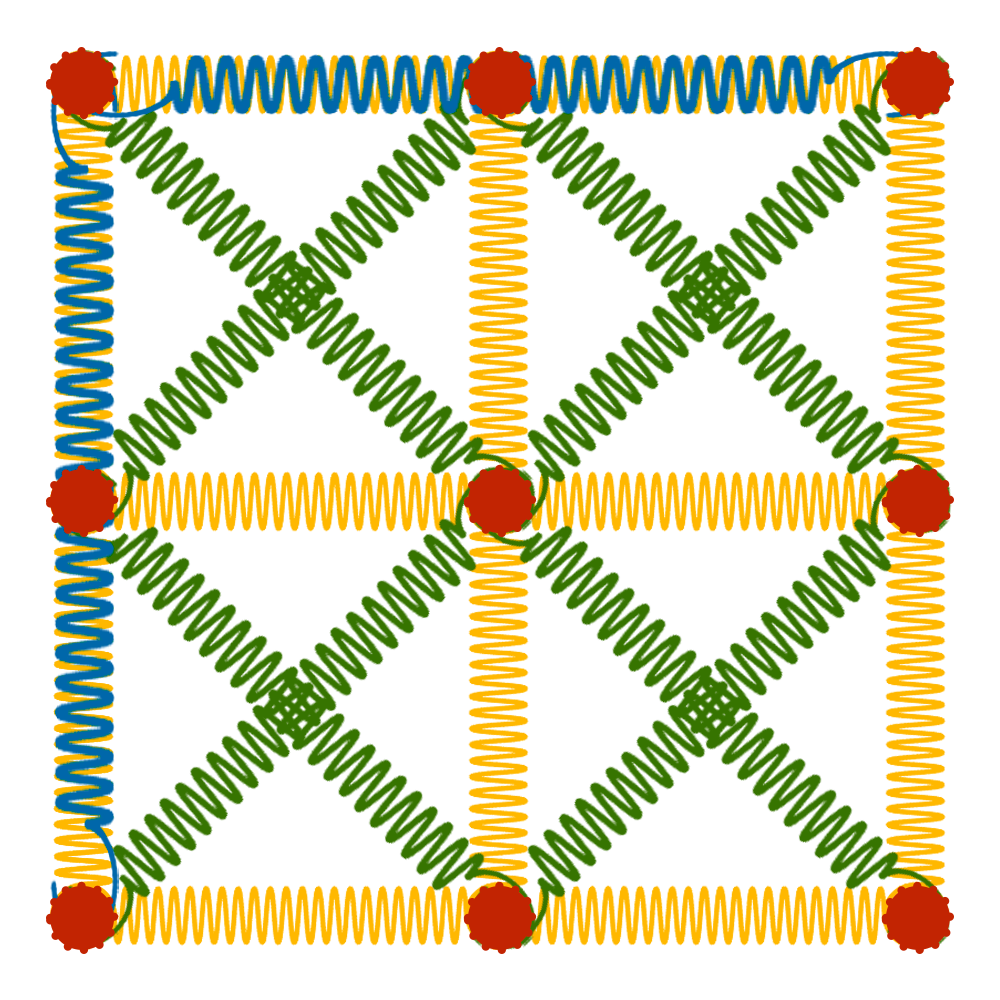
\includegraphics[width=0.5\textwidth]{img/structures.png};
    \caption{Esquema de las estructuras}
    \label{fig:structures}

\end{figure}

\subsubsection{Estructura Structural}\label{sec:estructura-estructural}
Esta estructura se basa en muelles que conectan las partículas con sus vecinas en las direcciones horizontal y vertical. Sin esta, la malla no se mantiene unida.
\begin{lstlisting}[language=Java, frame=single]
void addStructuralSprings()
{
    for (int i = 0; i < _numNodesH; i++)
    {
        for (int j = 0; j < _numNodesV; j++)
        {
            if (i < _numNodesH - 1)
            _springs.add(new DampedSpring(_nodes[i][j], _nodes[i+1][j], Ke, Kd));
            if (j < _numNodesV - 1)
            _springs.add(new DampedSpring(_nodes[i][j], _nodes[i][j+1], Ke, Kd));
        }
    }
}
\end{lstlisting}

\subsubsection{Estructura Shear}\label{sec:estructura-shear}
Esta estructura se basa en muelles que conectan las partículas con sus vecinas en las direcciones diagonal.

\begin{lstlisting}[language=Java, frame=single]
void addShearSprings()
{
    for (int i = 0; i < _numNodesH; i++)
    {
        for (int j = 0; j < _numNodesV; j++)
        {
        if ((i < _numNodesH - 1) && (j < _numNodesV - 1))
            _springs.add(new DampedSpring(_nodes[i][j], _nodes[i+1][j+1], Ke, Kd));
        if ((i < _numNodesH - 1) && (j > 0))
            _springs.add(new DampedSpring(_nodes[i][j], _nodes[i+1][j-1], Ke, Kd));
        }
    }
}
\end{lstlisting}

\subsubsection{Estructura Bend}\label{sec:estructura-bend}
Esta estructura se basa en muelles que conectan las partículas con sus vecinas en las direcciones horizontal y vertical a dos posiciones de distancia.

\begin{lstlisting}[language=Java, frame=single]
void addBendSprings()
{
    for (int i = 0; i < _numNodesH; i++)
    {
        for (int j = 0; j < _numNodesV; j++)
        {
        if (i < _numNodesH - 2)
            _springs.add(new DampedSpring(_nodes[i][j], _nodes[i+2][j], Ke, Kd));
        if (j < _numNodesV - 2)
            _springs.add(new DampedSpring(_nodes[i][j], _nodes[i][j+2], Ke, Kd));
        }
    }
}
\end{lstlisting}

\subsubsection{Muelle con amortiguamiento}\label{sec:muelle-amortiguado}

Para simular la fricción en el sistema, se añade una fuerza de amortiguamiento lineal a la fuerza elastica de los muelles. Esta fuerza se calcula como el producto de la tasa de cambio de la elongación por un coeficiente de amortiguamiento.

\begin{lstlisting}[language=Java, frame=single]
    float _lanterior = _l;
    _e = PVector.sub(_p2.getPosition(), _p1.getPosition());
    _l = _e.mag();
    _eN = _e.normalize(null);
    _v = (_lanterior - _l) / simStep;

    PVector Fe = _eN.copy().mult(_Ke * (_l - _l0));
    PVector Fd = _eN.copy().mult(-_Kd * _v);

    _F = PVector.add(Fe, Fd);
\end{lstlisting}


\subsection{Malla deformable por funciones}\label{sec:malla-funcion}

Para conseguir que la malla se deforme, se generan funciones de onda que se aplican a los vértices de la malla. Al código propircionado se le implementan las funciones de onda y se le añade colision a la malla creando partículas en las mismas posiciones de los vertices de la textura.

\begin{lstlisting}[language=Java, frame=single]

void updatePositions(float [][][] pos){
        int index = 0;
        for (int i = 0; i < mapSize; i++){
                for (int j = 0; j < mapSize; j++){
                        particles.get(index).setPosition(
                            new PVector (
                                pos[i][j][0], 
                                pos[i][j][1], 
                                pos[i][j][2]));
                        index++;
                    }
            }
    }
\end{lstlisting}

Para simular un efecto real, se deja caer una bola y se comprueban las colisiones con estas particulas que son invisibles. De esta forma se consigue que la malla interactue con la pelota como si estubiera flotando en el mar.

\section{Ejercicio 1: Simulación Dinámica de un Objeto Deformable Sólido}\label{sec:ejercicio1}

En esta primera parte veremos la simulación de un objeto deformable de tipo malla en forma de portería donde constará de 
4 redes: dos laterales, la parte superior y la parte frontal. Cada una de estas redes estará compuesta por una serie de muelles que conectan las partículas entre sí.

Para poder unir las redes entre sí, podemos asumir que algunos de los nodos de lamisma son nodos que no se mueven y que se encuentran en la misma posición que los nodos de las redes adyacentes. 
De esta forma, se pueden unir las redes entre sí mediante muelles que conectan los nodos de una red con los nodos de la red adyacente.

Para poder simular los muelles, utilizaremos muelles con amortiguamiento lineal.

\subsection{Resultados y Análisis}\label{sec:fb-resultados}

Enlace al video de la simulación: \url{}
Las diferencias de comportamiento que se pueden ver entre los tipos de disposiciones de muelles de la malla son las siguientes:
\begin{itemize}
    \item Estructura Structural: La malla se mantiene unida en todas las direcciones. Esto significa que cada nodo en la malla está conectado a todos sus vecinos inmediatos en todas las direcciones: arriba, abajo, izquierda y derecha.
    \item Estructura Shear: La malla se mantiene unida en todas las direcciones diagonales. En este caso, cada nodo está conectado a sus vecinos en las direcciones diagonales, lo que permite una mayor flexibilidad en la deformación de la malla.
    \item Estructura Bend: La malla se mantiene unida en todas las direcciones a dos posiciones de distancia. Esto significa que cada nodo está conectado no solo a sus vecinos inmediatos, sino también a los nodos que están a dos posiciones de distancia. Esto permite una mayor resistencia a la flexión y la torsión.
\end{itemize}

En cuanto al comportamiento de la simulación, se puede observar que cambia significativamente en función de la disposición de los muelles en la malla. 
Por ejemplo, en el caso de la estructura Structural, la malla se mantiene unida en todas las direcciones, lo que significa que es más rígida y 
menos flexible que en los otros casos. 
Por otro lado, en el caso de la estructura Shear, la malla es más flexible y puede deformarse en direcciones diagonales, lo que permite 
una mayor variedad de movimientos. 
En el caso de la estructura Bend, la malla es más resistente a la flexión y la torsión, lo que significa que es más difícil de deformar en estas direcciones.

Enlace al video de la simulación: \url{}
2- explica qué efecto tiene incrementar o disminuir el parámetro en
cuestión, y por qué.

La complejidad computacional de las disposiciones de muelles puede variar dependiendo de la estructura de la malla y del algoritmo utilizado para la simulación. Aquí hay una descripción general de la complejidad computacional de cada disposición:
\begin{itemize}
    \item Estructura Structural: La complejidad computacional es generalmente de orden O(n), donde n es el número de nodos en la malla. Esto se debe a que cada nodo está conectado a un número constante de vecinos (generalmente 4 en una malla 2D), y por lo tanto el tiempo de computación es lineal en el número de nodos.
    \item Estructura Shear: La complejidad computacional también es de orden O(n), por las mismas razones que la estructura Structural. Aunque cada nodo está conectado a más vecinos (8 en una malla 2D), el número de vecinos sigue siendo constante, por lo que el tiempo de computación es lineal en el número de nodos.
    \item Estructura Bend: La complejidad computacional puede ser mayor en este caso, dependiendo de cómo se implemente la simulación. Si se utiliza un algoritmo simple que recorre cada par de nodos conectados, la complejidad podría ser de orden O(n^2), donde n es el número de nodos. Sin embargo, con una implementación más sofisticada que aproveche la estructura de la malla, la complejidad podría reducirse a O(n).
\end{itemize}


\section{Ejercicio 2: Simulación Cinemática de Olas}\label{sec:ejercicio2}

En esta segunda parte veremos la simulación de olas. Para ello, se utilizará una estructura llamada mapa de alturas.
Este mapa de alturas consiste en un conjunto de puntos con 3 coordenadas distribuidos homogéneamente en un plano.

Para simular las olas hemos utilizado tres tipos de ondas:
\begin{itemize}
    \item Onda radial: la perturbación se propaga en todas direcciones.
    \item Onda direccional: la perturbación se propaga en una dirección concreta.
    \item Onda Gerstner: la perturbación se propaga en una dirección concreta y tiene una forma sinusoidal.
\end{itemize}

\subsection{Resultados y Análisis}\label{sec:fb-resultados2}

Enlace al video de la simulación: \url{}

\newpage
\section{Conclusiones}\label{sec:conclusion}


\end{document}